\section{Results}\label{sec:results}

This section presents and discusses the results of our study using the \cds  (4,076 pairs). We evaluate it from the following aspects: malware detection performance for each strategies, \mas and \net (Section~\ref{sec:comparison}). Then, we detail the results of combining both approaches, highlighting where they can complement each other (Section~\ref{sec:strategy}). Finally, we present the detection rates for each malware family, as well as the performance on unknown families (Section~\ref{sec:family}). We remind the reader that all results presents at Sections above are based on Random Forest approach, since it delivered the best performance, as present at next Section (Section~\ref{sec:ml}).

\subsection{Comparison of Machine Learning Algorithms}\label{sec:ml}

In this section, we present the performance of popular machine learning algorithms to determine which model could better support the \mas in malware detection. We also explore a novel classifier algorithm called the Energy-Based Flow Classifier (EFC)~\cite{DBLP:journals/tnsm/PontesSGBM21}, which offers certain advantages over traditional machine learning algorithms, such as the ability to infer a model using only benign traffic samples~\cite{DBLP:journals/tnsm/PontesSGBM21}, eliminating the need to label malicious samples.

For the comparison of popular classification algorithms, we selected several techniques, including Random Forest, Linear Discriminant Analysis (LDA), Quadratic Discriminant Analysis (QDA), and Logistic Regression. To find the best-fitting model, we varied multiple parameters and used cross-validation to maximize the performance of each machine learning algorithm.

Figure~\ref{fig:metrics} shows that the trained models from different algorithms exhibit varying performance results. Overall, the study show that the Random Forest algorithm outperforms the others algorithms, achieving higher values across the explored metrics: recall, precision, \fone, and Area Under the Curve (AUC).

\begin{finding}
  The Random Forest algorithm outperforms the others popular classification algorithms, achieving higher values across the metrics explored (recall, precision, \fone, and Area Under the Curve).
\end{finding}


\begin{figure*}[h]
  \centering
  
    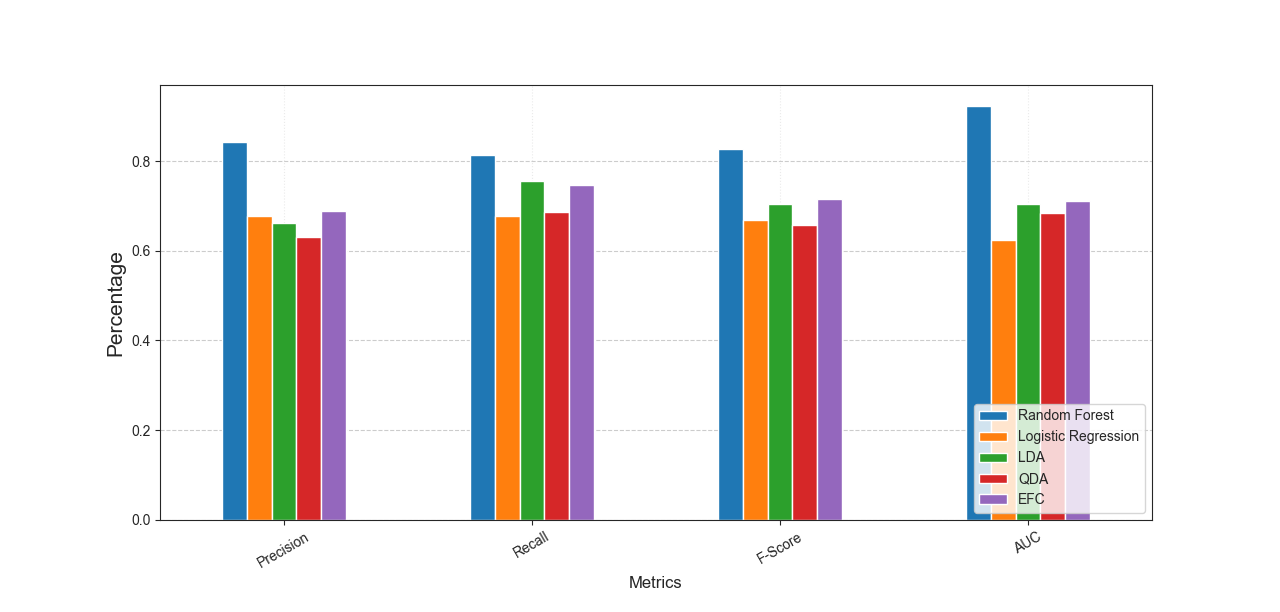
\includegraphics[width=0.85\textwidth]{image/barGraphMetrics.png} \\[\abovecaptionskip]
    
  \caption{The comparison of machine learning algorithms}\label{fig:metrics}
\end{figure*}


\subsection{Comparison of two detection Strategy}\label{sec:comparison}

{\bf \mas.} Considering the \cds (4,076 apps), the \fhc present
a total of {$1,395$} repackaged apps flagged as malware ({$34.22$\%} of the total number of repackaged apps), for which the repackaged app version calls at least one additional sensitive API. They explore accuracy metrics (such as Precision, Recall, and F-measure ($F_1$)), taking advantage of \vt to label the \cds and building a ground truth. Table~\ref{tab:accuracy} summarize the result of their study (First row). The study indicate that the \mas achieves an accuracy of 0.54 when considering the \cds. Nonetheless, the \mas fails to correctly classify $1,720$ assets as malware on the \cds (FN column, first row of Table~\ref{tab:accuracy}), and wrongly labeled the repackaged version of $220$ apps as malware (FP column). Therefore, the study reveals a {\bf lower performance} related to the accuracy of the approach, indicating that when considering the \cds, the accuracy of the \mas using DroidBot as test generate tool is just over $50$\%.

{\bf Flow Analysis.} Surprisingly, also considering the \cds (\apps pairs), we explored Flow Analysis with machine learning algorithm (Random Forest). As described in Section~\ref{sec:learning}, we trained $70$\% of the samples and tested on $30$\% of samples different from the trained ones. Our \cds cover \apps pair with $2,969$ original apps and $2,918$ malicious apps, totaling $5,887$ balanced samples. Accordingly, we trained our model on $4,120$ samples ($70$\% of $5,887$), and applied the trained model to $1,767$ samples ($30$\% of $5,887$). The Flow Analysis labeled a total of $690$ apps as malware, failed to correctly label $124$ assets as malware, and wrongly labeled the repackaged versions of $175$ samples (second row of Table~\ref{tab:accuracy}). Our Flow Analysis had a better performance, when compared to \mas, with an accuracy rate of $82$\%. From these results, we can conclude that Flow Analysis could be a complementary technique to \mas, improving the identification of malicious code in Android apps. In the next section, we present the results of combining both techniques for suspicious app detection.

\begin{finding}
The experimental results demonstrate that Network Flow analysis, combined with a machine learning algorithm, outperforms the \mas, with \fone of $0.82$. This proves to be an effective strategy to support the \mas for malware identification.
\end{finding}


\begin{table*}[h]
  \caption{Accuracy of both strategy on \cds.}
\centering{
  \begin{tabular}{lrrrrrr} \hline
    Dataset & TP   & FP  & FN  & Precision & Recall & $F_1$ \\
    \hline
    
    %\mas + Traces  & \sds (102)   & 67   & 18  & 2   & 0.78      & 0.97   & 0.87  \\
    \fhc : \mas (4,076 pairs)    & 1,175  & 220 & 1,720 & 0.84       & 0.40   & 0.54  \\
    Flow Analysis (1767 samples)~\footnote{Using Random Forest as ML algorithm}    & 690   & 175   & 124   & 0.79      & 0.84   & 0.82  \\
    %\mas + Traces  & \cds (1203)   & 214  & 326 & 245 & 0.39      & 0.46   & 0.42  \\ 
    \mas and Flow Analysis (4,076 pairs)    & 2,712   & 334   & 183   & 0.89      & 0.93   & 0.91  \\
    \hline
  \end{tabular}
  }
  \label{tab:accuracy}
\end{table*}


\subsection{Combining both Strategy}\label{sec:strategy}

Finally, to confirm our hypothesis from Section~\ref{sec:comparison}, we investigated the benefits of combining both approaches (\mas and Flow Analysis). The combined execution of both techniques correctly classified $2,712$ repackaged apps as malware (TP) and significantly decreased the number of (FN) from $1,720$ to $183$. However, this execution increased the number of (FP) from $220$ to $334$. The combination of both techniques proved to be more effective than the vanilla \mas. In summary, the results reveal that the combination of both techniques achieves an accuracy rate of $91$\% (third row of Table~\ref{tab:accuracy}).

To understand the benefits of each method, we further analyze the contribution of them for the accuracy. We report the raise of True Positive (TP) and False Positive (FP) for each technique in Figure~\ref{fig:venn}. The figure reveal that different approaches present different contribution to the final detection result.

\begin{finding}
When combining both techniques, we improve the overall accuracy (\fone) of \mas at malware detection, from $0.54$ to $0.91$ at \cds.
\end{finding}

\begin{figure}[t!]
  \centering
  \begin{tabular}{@{}c@{}}
    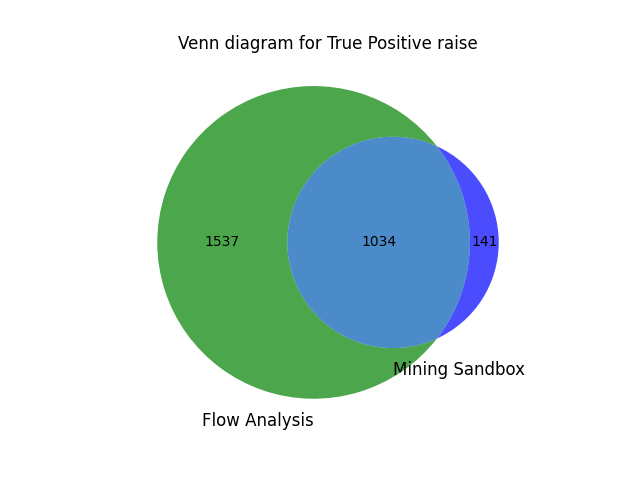
\includegraphics[width=0.54\textwidth]{image/vennTP.png} \\[\abovecaptionskip]
    \small (a) True Positive raise
  \end{tabular}

  \begin{tabular}{@{}c@{}}
    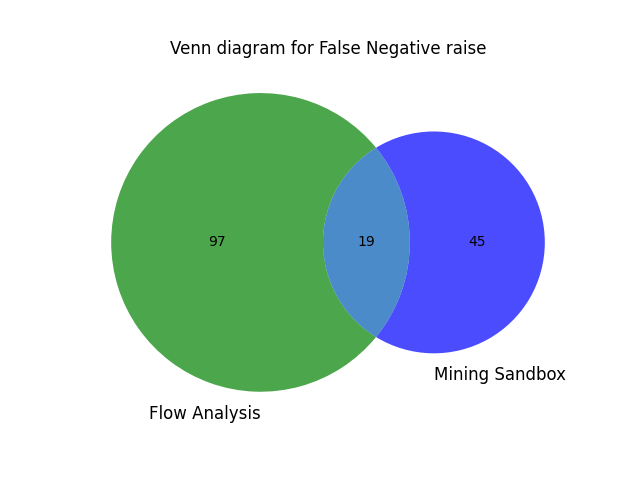
\includegraphics[width=0.54\textwidth]{image/vennFP.png} \\[\abovecaptionskip]
    \small (b) False Positive raise
  \end{tabular}

  \caption{Contribution to the final detection result}\label{fig:venn}
\end{figure}






\subsection{Detection Performance based on Malware Family}\label{sec:family}

In this section, we present the performance of our experiment based on each malware family. Since the number of samples in one family differs from the number in another, the overall detection rate is influenced more by the families with larger sample sizes. However, our results become inconsistent if we use the same number of samples for each family. To resolve the paradox, we present the results of the actual number of samples from the $10$ most representative families, which account for $87.83\%$ of all samples (Section~\ref{sec:familyDetection}). We also explored the detection rate of suspected recent malware samples. Although their families are unknown, we demonstrated that it is possible to improve the detection rate of suspicious apps by combining both strategies (Section~\ref{sec:unknowfamily}).


\subsubsection{Detection rate of 10 most representative malware families}\label{sec:familyDetection}

Among the $10$ most representative families, combining both strategies, the families with the highest earnings are \tjk and \gps. Regarding \tjk family malware, among the 34 samples evaluated, the \fhc flagged only 2 apps ($5.88$\%) as malicious. However, when combined with Flow Analysis, both approaches correctly labeled $32$ assets ($94.11$\%) as malicious, marking an $88.23$\% increase. Despite this, the \tjk family does not have as many representative samples as the \gps family, which accounts for $32.80$\% of all samples in the \cds, with $1,337$ samples. Among them, the \mas flagged $334$ samples ($12.93$\%) as malicious, while the combination of them indicated that $1,275$ ($95.36$\%) had suspicious activity, representing an $82.42$\% increase. Malware belonging to the \gps family automatically connects to networks, communicates with remote servers, and downloads and installs other apps or adware without the user’s knowledge\cite{DBLP:journals/jnca/WangCYYPJ19}. Due to their high network interaction, they are more easily detected by \net, proving it to be more efficient in detecting samples with malicious network behaviors.

Still, we should also note that $2$ families can correctly identified all samples as malware just with the \mas, \fm{airpush} and \fm{leadbolt}, with $120$ and $43$ samples respectively. At this case, the \net do not contribute to improving the ability to detect malicious activity, and just confirms the  maliciousness of the samples. The result reveals that the \mas remain effective for certain malware families. Figure~\ref{fig:bar} shows the detection performance of our strategies for the $10$ most representative families. In the figure, we can see that samples for the \gps family, had the the greatest benefit of the malware detection rate, with the support of flow analysis.



\begin{figure*}[h]
  \centering
  
    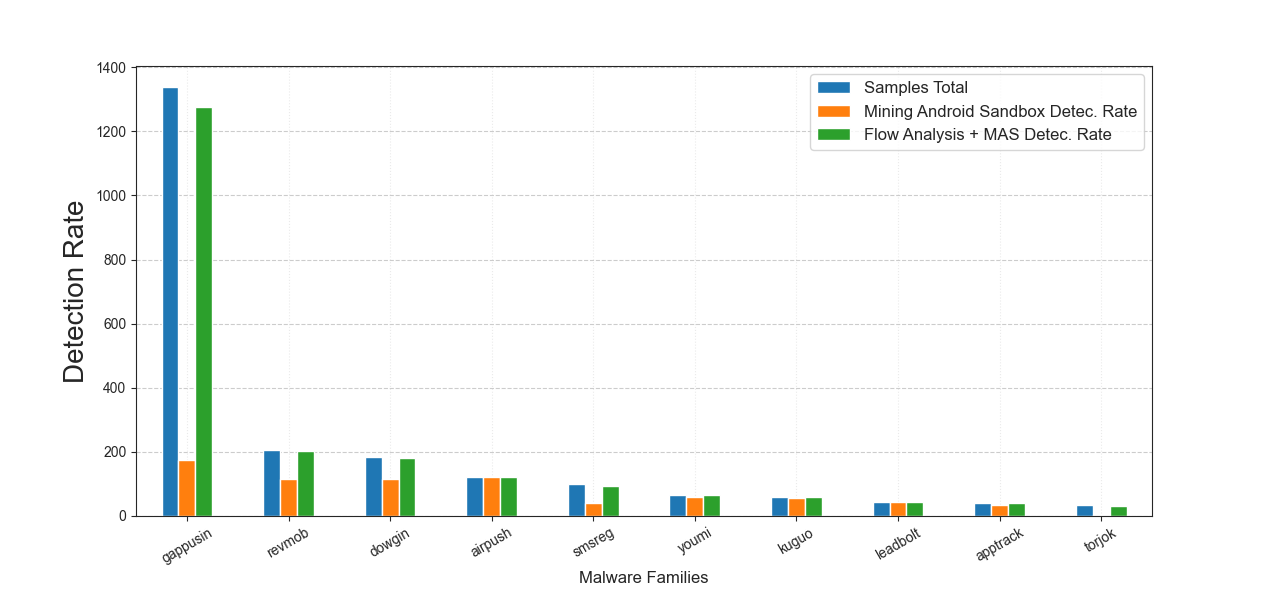
\includegraphics[width=\linewidth]{image/barGraph.png} \\[\abovecaptionskip]
    
  \caption{Detection Rate for Family}\label{fig:bar}
\end{figure*}

\begin{finding}

The combination of the \mas with \net, improve the malware detection rate for the \gps family (from $12.93$\% to $95.36$\%), the most representative family in \cds. This demonstrates the potential of this solution in detecting samples with malicious network behaviors.

\end{finding}


\subsubsection{Detection rate of unknown malware family}\label{sec:unknowfamily}

According to \vt, among the samples from our \cds, at least two \ses identified $253$ samples as malware. However, they were unable to specify their families. Since new malware emerges daily, accurately classifying recent malicious apps into their respective families is both challenging and time-consuming~\cite{DBLP:journals/compsec/WangTW21,DBLP:journals/compsec/ContiKP22}, which suggests that these are recent malware.

Although the specific families are unknown, the \mas detected suspicious activity in $114$ samples ($45.05$\%) from this set. On the other hand, when focusing solely on the results from the \net, for these unknown malware families, $124$ samples ($49.01$\%) were flagged as malicious. When we combine both approaches, the total number of apps flagged for suspicious activity increases to $170$ ($67.19$\%). Based on these results, we conclude that \net can effectively support the \mas, even for recently identified malicious apps, without malware family classification at the time of this research.

\begin{finding}

Even for recently malicious apps with unknown malware families, \net can support the \mas to improve the detection rate of apps with suspicious activities.

\end{finding}